\clearpage
\section{Installation Sensor}\label{sec:Sensor}

Das Sensor-Bord ist die physikalische Schnittstelle, wo Aktionen ausgelöst werden und anschliessend von Openhab empfangen und verarbeitet werden.
\subsection{Anleitung einrichten}
\begin{figure}[H]
	\begin{center}
		\begin{minipage}[b]{.3\linewidth} % [b] => Ausrichtung an \caption
			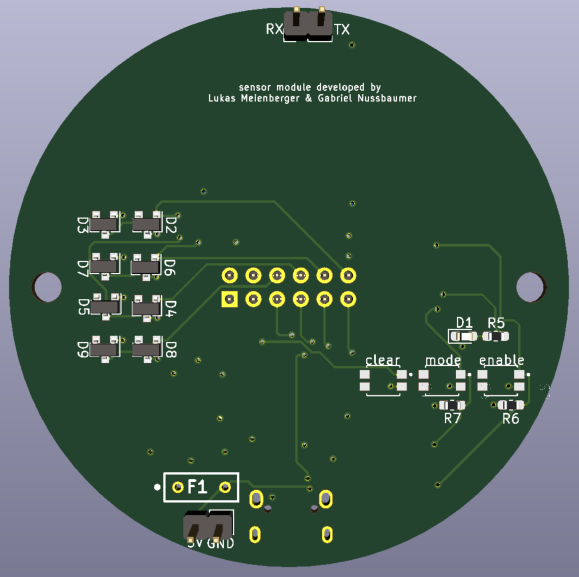
\includegraphics[width=\textwidth]{graphics/Sensor1.PNG}
			\caption{Sensor-Bord Rückseite}
			\label{pic: Sensorbord}
		\end{minipage}
		\hspace{.1\linewidth}% Abstand zwischen Bilder
		\begin{minipage}[b]{.3\linewidth} % [b] => Ausrichtung an \caption
			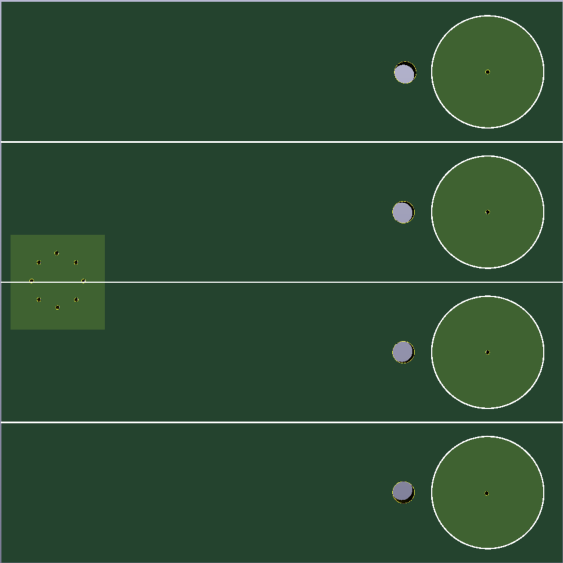
\includegraphics[width=\textwidth]{graphics/Sensor3.PNG}
			\caption{Frontprint}
			\label{pic: Frontprint}
		\end{minipage}
	\hspace{.1\linewidth}% Abstand zwischen Bilder
		\begin{minipage}[b]{.3\linewidth} % [b] => Ausrichtung an \caption
	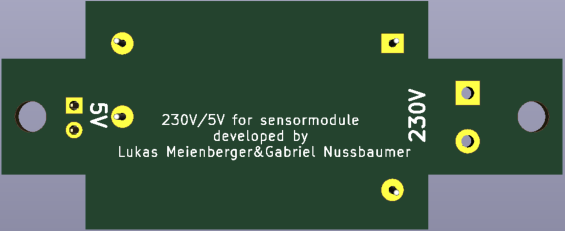
\includegraphics[width=\textwidth]{graphics/Sensor2.PNG}
	\caption{Spannungsversorgung Rückseite}
	\label{pic: ruckseite}
\end{minipage}
\end{center}
\end{figure}

\begin{enumerate}
	\item Die Installation ist in einem spannungslosen Zustand durchzuführen.\\
	\\
	\item An der Rückseite von der Spannungsversorgung wird die Netzspannung 230\,VAC angeschlossen siehe Abbildung \ref{pic: ruckseite}.\\
	\\
	\item Das Sensor-Bord \ref{pic: Sensorbord} wird mit der Spannungsversorgung \ref{pic: ruckseite} und wird mit einem Standard Feller Gr-1 Befestigungsrahmen in eine Vorgesehene Einbauschalteröffnung eingebaut. \\
	\\
	\item Der Frontplatte \ref{pic: Frontprint} wird mit dem Abdeckrahmen Gr-1 auf das Sensor-Bord \ref{pic: Sensorbord} gesteckt. Die Beschriftung der Pins, GND zu GND ist dringend zu Beachten beim zusammenstecken, es kann auch auf den Markierungspunkt beim Stecker geachtet werden.\\
	\\
	\end{enumerate}

\subsection{Inbetriebnahme}
Sobald das Sensor-Board mit Spannung versorgt wird, startet das Config-Portal des Bords. Mit einem beliebigen Gerät kann im nach einem WLAN-Netzwerk gesucht werden. Das Netzwerk hat den Namen 'Sensor' gefolgt von der 10 Stelligen Chip-ID des Mikrocontrollers. 

Mit der Funktion 'Scan WiFi' werden vorhanden Netzwerke angezeigt. Wird ein eigener MQTT Server installiert, kann an dieser Stelle die IP-Adresse angegeben werden und der Port ist Default '1883' anzugeben. Die Eingabe bei 'board location' wird verwendet um MQTT-Topics zu generieren, sie muss eindeutig sein. Werden mehrere Sensor-Bords verbaut, unterscheiden sie sich an der 'bord location'. Mit dem Button 'save' werden die Eingaben gesichert und müssen bei einem erneuten Start nicht mehr eingegeben werden. Kann sich das Sensor-Board erfolgreich ins Lokale Netzwerk anmelden, blinkt die Status LED in einem regelmässigen Zyklus. Bei jeder Zustandsänderung der Statusleuchte, wird eine Temperaturmessung mit dem NTC-Widerstand durchgeführt. 

\subsection{Programmierung}
Verschiedene Eigenschaften können mit dem Entwicklertool zusätzlich verändert werden, falls der Programmcode des Mikrocontrollers bearbeitet wird. In der nachfolgenden Tabelle sind die wichtigsten Default-Konfigurationen enthalten.
\begin{table}[H]
	\centering
	\begin{tabular}{|l|l|l|}
		\hline 
		Bezeichnung & Variable & Wert \\ 
		\hline 
		Zeit Intervall Messungen & NUM\_SEC & 10 \\ 
		\hline 
		Allgemeiner MQTT-Topic  & MQTT\_SERIAL\_PUB& data/sensorboard/ \\ 
		\hline 
		Offset Temperatur Messung & b\_temp & 0.1369856 \\ 
		\hline  
		Steigung Temperatur Messung & m\_temp & 0.0008155002 \\ 
		\hline  
		Treshold Trigger Touchsensor & tresh& 15 \\ 
		\hline
		Messungen für Mean Wert Temperatur & I & 10 \\ 
		\hline  
		Messungen für Mean Wert Touchwert & count & 15 \\ 
		\hline  
	\end{tabular} 	
\end{table}
\subsection{Netzwerkeinstellungen ändern}
Soll sich das Sensor-Board in ein anderes Netzwerk anmelden,gibt es zwei verschiedene Möglichkeiten die Einstellungen zu ändern. Wenn während des Startvorgangs die Clear-Taste 5\,s betätigt wird, eröffnet der Mikrocontroller das Config-Portal. Das Config-Portal wird ebenfalls geöffnet, wenn das einst eingetragene Netzwerk nicht mehr gefunden wird und keine Verbindung hergestellt werden kann.
\subsection{System Tasten}
Mit der Taste 'enable' wird manuell ein Neustart durchgeführt. \\
Mit der Taste 'clear' wird während dem Startvorgang das Config-Portal eröffnet. \\
Die Taste 'mode' hat auf dem Prototyp Sensor-Bord keine Funktion.
\subsection{Topics}
In der Nachfolgenden Tabelle sind die Automatisch generierten Topics, welche weiter in Openhab verwendet werden. Als location wurde im Config-Portal 'location' eingetragen.
\begin{table}[H]
	\centering
	\begin{tabular}{|l|l|}
		\hline 
		Topic  & Funktion  \\ 
		\hline 
		data/sensorboard/location/S1 & Taster 1 wurde betätigt  \\ 
		\hline
		data/sensorboard/location/S2 & Taster 2 wurde betätigt  \\ 
		\hline
		data/sensorboard/location/S3 & Taster 3 wurde betätigt  \\ 
		\hline
		data/sensorboard/location/S4 & Taster 4 wurde betätigt  \\ 
		\hline
		data/sensorboard/location/S0 & Gemessene Raumtemperatur  \\ 
		\hline
			\end{tabular} 	
	\label{tab: MQTT-Topics Sensor}
	\caption{MQTT-Topics}
\end{table}

